\subsection{Traceability Between Test Cases and Requirements}
In the traceability graphs, test suites appear at the tail of an arrow and
requirements appear at the head. In the traceability matrices, the test suites
related to a requirement's verification are marked with an ``X'' in the
requirement's column.

\vspace*{\fill}
\begin{figure}[tbh]
    \centering
    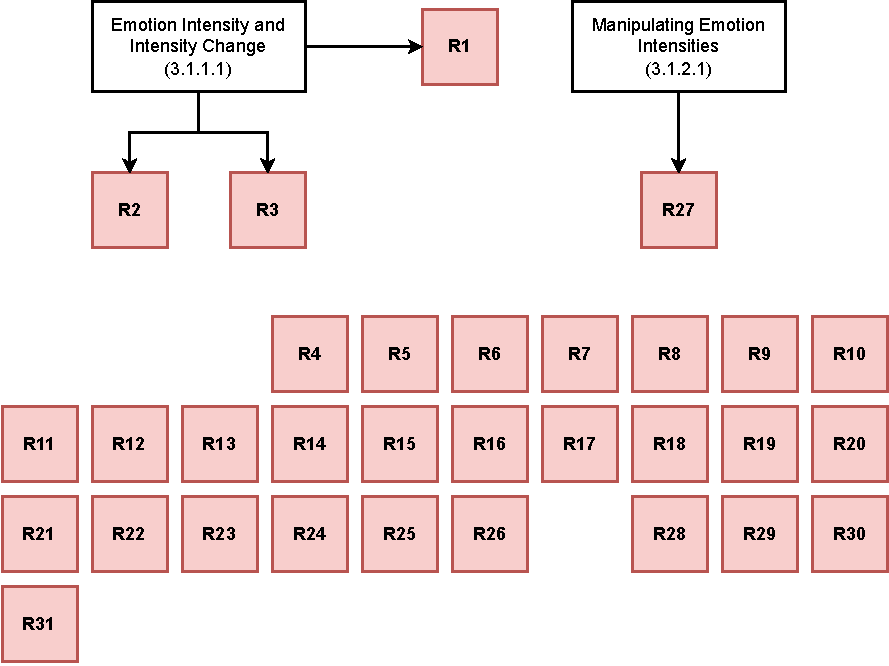
\includegraphics[width=0.9\linewidth]{figures/testSuites2funreqs.pdf}
    \caption{Traceability between System and Integration-Level Test Suites and
    Functional Requirements}
    \label{fig:traceSystemTS2FunReqs}
\end{figure}
\vspace*{\fill}

\begin{landscape}
    \vspace*{\fill}
    \begin{table}[tbh]
        \centering
        \resizebox{\linewidth}{!}{%
            \begin{tabular}{|c|c|c|c|c|c|c|c|c|c|c|c|c|c|c|c|c|c|c|c|c|c|c|c|c|c|c|c|c|c|c|c|}
                \hline
                & \rref{R_Types} & \rref{R_IntensityTypeUse} &
                \rref{R_IntensityChangeType} & \rref{R_IntensityDecayType} &
                \rref{R_EmotionKindsType} & \rref{R_EmotionStateType} &
                \rref{R_EmotionDecayStateType} & \rref{R_EmotionType} &
                \rref{R_PADPointType} & \rref{R_TimeType} & \rref{R_WorldType}
                & \rref{R_WorldChangeType} & \rref{R_DistanceType} &
                \rref{R_DistanceChangeType} & \rref{R_GoalType} &
                \rref{R_PlanType} & \rref{R_SocialAttachment} &
                \rref{R_Attention} & \rref{R_MixingEmotionsPES} &
                \rref{R_PartitionEmotions} & \rref{R_MixingEmotionsCTE} &
                \rref{R_GenerateEmotionCTE} & \rref{R_CalculateIntensity} &
                \rref{R_DecayIntensity} & \rref{R_DecayEmotion} &
                \rref{R_NewESFromDecay} & \rref{R_UpdateAnIntensity} &
                \rref{R_UpdateEmotionState} & \rref{R_UpdateEmotion} &
                \rref{R_GetEmotionState} & \rref{R_Convert2PAD} \\\hline

                \ref{sec_IntensityAndIntensityChg}.1 & X & X & X
                &&&&&&&&&&&&&&&&&&&&&&&&&&&& \\\hline

                \ref{sec:sys-methods-emotionintensity}.1 &  &  &
                &&&&&&&&&&&&&&&&&&&&&&&& X &&&& \\\hline

            \end{tabular}%
        }
        \caption{Traceability between System and Integration-Level Test Suites
            and Functional Requirements}
        \label{tab:traceSystemTS2FunReqs}
    \end{table}
    \vspace*{\fill}
\end{landscape}

\vspace*{\fill}
\begin{figure}[tbh]
    \centering
    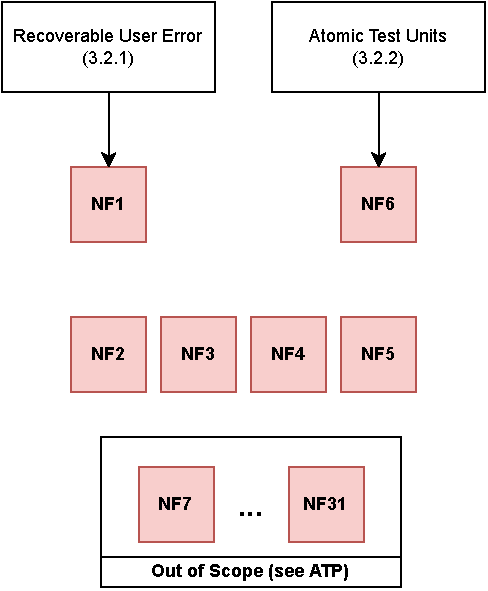
\includegraphics[width=0.5\linewidth]{figures/testSuites2nonfunreqs.pdf}
    \caption{Traceability between System and Integration-Level Test Suites and
        Nonfunctional Requirements}
    \label{fig:traceSystemTS2NonfunReqs}
\end{figure}
\vspace*{\fill}

\begin{table}[tbh]
    \centering
    \begin{tabular}{|c|c|c|c|c|c|c|}
        \hline
        & \nfref{N_RecoverNeutral} & \nfref{N_RecoverNoChange} &
        \nfref{N_Speed} & \nfref{N_Complex} & \nfref{N_Efficient} &
        \nfref{N_Atomic} \\\hline

        \ref{sec:sys-nf-recover} & X &  &  &&& \\\hline

        \ref{sec:sys-nf-atomic} &  &  &  &&& X \\\hline

    \end{tabular}
    \caption{Traceability between System and Integration-Level Test Suites
        and Nonfunctional Requirements}
    \label{tab:traceSystemTS2NonfunReqs}
\end{table}
\vspace*{\fill}